\documentclass[11pt,a4paper]{article}

\usepackage[utf8]{inputenc}
\usepackage[T1]{fontenc}
\usepackage[english]{babel}
\usepackage[a4paper,margin=2.4cm]{geometry}

\usepackage{amsmath, amssymb, amsthm}
\usepackage{mathtools}
\usepackage{stmaryrd}
\usepackage{booktabs}
\usepackage{tabularx}
\usepackage{array}
\usepackage{caption}
\usepackage{subcaption}
\usepackage{float}
\usepackage{enumitem}
\usepackage{microtype}
\usepackage{xcolor}
\usepackage{listings}
\usepackage{fancyhdr}
\usepackage{titlesec}
\usepackage{graphicx}
\usepackage{tikz}
\usetikzlibrary{positioning, arrows.meta, fit, backgrounds, calc, shapes.geometric}
\usepackage[hidelinks]{hyperref}

%  ---  Palette shared with the companion reports  ---
\definecolor{ink}{RGB}{26,30,36}
\definecolor{slate}{RGB}{92,101,112}
\definecolor{mist}{RGB}{233,235,238}
\definecolor{rulegrey}{RGB}{188,194,201}
\definecolor{steel}{RGB}{47,72,102}
\definecolor{steellight}{RGB}{124,146,172}
\definecolor{signal}{RGB}{160,32,45}
\definecolor{southc}{RGB}{51,115,204}
\definecolor{northc}{RGB}{230,128,38}
\definecolor{knows}{RGB}{26,140,70}

\hypersetup{
    colorlinks=true,
    linkcolor=steel,
    citecolor=steel,
    urlcolor=steel,
    pdftitle={The Coordinated Attack on a Warehouse Floor: Common Knowledge as an Action Precondition},
    pdfauthor={Haniel Ulises},
}

\color{ink}

\setlength{\headheight}{22pt}
\pagestyle{fancy}
\fancyhf{}
\fancyhead[L]{\small\textcolor{slate}{\itshape The Coordinated Attack on a Warehouse Floor}}
\fancyhead[R]{\small\textcolor{slate}{\thepage}}
\renewcommand{\headrulewidth}{0.4pt}
\renewcommand{\headrule}{\hbox to\headwidth{\color{rulegrey}\leaders\hrule height \headrulewidth\hfill}}

\titleformat{\section}{\normalfont\large\bfseries\color{ink}}{\thesection}{0.7em}{}
\titleformat{\subsection}{\normalfont\normalsize\bfseries\color{ink}}{\thesubsection}{0.7em}{}
\titleformat{\paragraph}[runin]{\normalfont\bfseries\color{slate}}{}{0em}{}[.]

\captionsetup{font=small, labelfont={bf,color=slate}, textfont=footnotesize}

\theoremstyle{definition}
\newtheorem{definition}{Definition}
\newtheorem{proposition}{Proposition}
\newtheorem{lemma}{Lemma}
\newtheorem{corollary}{Corollary}
\newtheorem{fact}{Fact}
\newtheorem{remark}{Remark}

\lstdefinestyle{sys}{
    backgroundcolor=\color{mist},
    basicstyle=\ttfamily\scriptsize\color{ink},
    keywordstyle=\color{steel}\bfseries,
    commentstyle=\color{slate}\itshape,
    stringstyle=\color{slate},
    morecomment=[l]{;},
    morekeywords={:types,:predicates,:objects,:agents,:goal,:init,:event,:action,:action-type,:observability-conditions,:precondition,:effects,:events,:relations,:designated,:conditions,:observability-types},
    frame=single,
    rulecolor=\color{rulegrey},
    framesep=5pt,
    xleftmargin=6pt,
    xrightmargin=0pt,
    breaklines=true,
    showstringspaces=false,
    columns=fullflexible,
    captionpos=b,
}
\lstset{style=sys}

%  ---  Notation  ---
\newcommand{\Ag}{\mathcal{A}}
\newcommand{\Mod}{\mathcal{M}}
\newcommand{\Ev}{\mathcal{E}}
\newcommand{\prd}{\otimes}
\newcommand{\Kop}[1]{K_{#1}}
\newcommand{\Eop}[1]{E_{#1}}
\newcommand{\Cop}[1]{C_{#1}}
\newcommand{\Kw}[1]{\mathit{Kw}_{#1}}
\newcommand{\code}[1]{\texttt{\small #1}}
\newcommand{\ag}[1]{\mathit{#1}}
\newcommand{\job}{\mathit{job}}
\newcommand{\pre}{\mathit{pre}}
\newcommand{\post}{\mathit{post}}
\newcommand{\dist}{\mathrm{dist}}
\newcommand{\depth}{\mathrm{depth}}
\newcommand{\atview}{\mathit{at\text{-}view}}
\newcommand{\sem}[1]{\llbracket #1 \rrbracket}

\begin{document}

\begin{titlepage}
\centering
\vspace*{2.4cm}
{\color{rulegrey}\rule{\textwidth}{0.8pt}}\\[0.9cm]
{\LARGE\bfseries The Coordinated Attack on a Warehouse Floor\par}
\vspace{0.5cm}
{\large\color{slate} Common Knowledge as an Action Precondition,\\
a Lossy Channel that Cannot Supply It, and a Signal that Can\par}
\vspace{0.7cm}
{\color{rulegrey}\rule{\textwidth}{0.8pt}}\\[1.4cm]

{\large Haniel Ulises\par}
\vspace{0.3cm}
{\color{slate} Epistemic Robotics}\\
\vspace{0.15cm}
{\color{slate}\today}

\vfill
{\color{slate}\small
Two robots must lift one load together, one under each end. A work order names
which of two stands, and only one robot can read it. Since an end raised alone
tips the load, each robot raises its end only if it knows the other raises the
other, and the weakest condition satisfying both is common knowledge of the
stand. The report states that condition as the precondition of an ontic action
in a dynamic epistemic planning domain, and asks which channel can establish it.

\vspace{0.6em}
A message over a channel that can lose it is given as an event model with three
events. We show that the product update with such a message preserves
$\mathrm{S5}$, and that it decreases the distance from the designated worlds to
a counterexample by at most one, so that each message adds at most one level of
mutual knowledge and no finite sequence of them yields common knowledge. On the
floor without a beacon this proves that no policy exists, for messages of any
number; the planner, on a bounded protocol, exhausts its space at depth five.
A stack light visible only from two viewpoints yields common knowledge in one
update, and only when both robots stand at their viewpoints. When a move is
witnessed only by the mover, the same signal yields one level of mutual
knowledge, as a message does, and the planner has the robots sight each other
first. Both floors were
executed in Gazebo through ePlanSys. Over the radio, four delivered messages
reached $E^4$ and the executor refused the lift; with the beacon, the policy
lifted the load from a joint start, with arrivals 0.40\,s apart.}
\vspace{1.2cm}
\end{titlepage}

\tableofcontents
\newpage

%  ======================================================================
\section{Scope}
\label{sec:scope}

The companion reports execute epistemic policies whose preconditions are
individual knowledge: a carrier crosses a bay it knows to be open, a robot
reports a site whose state it knows. This report concerns a precondition of a
different kind. The action is joint, and its precondition is common knowledge
of a group.

The problem is the coordinated attack of Gray~\cite{gray1978} and of Akkoyunlu,
Ekanadham and Huber~\cite{akkoyunlu1975}, in the form Halpern and Moses gave
it~\cite{halpern1990}: two parties must act simultaneously or not at all,
communicate over a channel that may lose messages, and cannot coordinate. It is
restated here as a warehouse task on the floor of the pass-through study, and
the result is obtained in three ways: by proof over the event models of the
domain, by exhaustive search of the planner, and by execution on simulated
robots.

Four claims are advanced.

\begin{enumerate}[leftmargin=1.4em, itemsep=2pt]
  \item A message over a lossy channel, as an event model, preserves
        $\mathrm{S5}$ and adds at most one level of mutual knowledge per
        message, whether or not it is delivered
        (Propositions~\ref{prop:s5} and~\ref{prop:onelevel}). On the floor
        without a beacon no sequence of actions of any length makes the lift
        applicable (Corollary~\ref{cor:radio}).
  \item A signal observed from viewpoints that are common knowledge yields
        common knowledge in one update, and the same signal observed by one
        robot yields no mutual knowledge at all
        (Propositions~\ref{prop:public} and~\ref{prop:alone}).
  \item The planner agrees with both results: it exhausts the radio floor and
        returns a policy of depth five on the beacon floor that does not use
        the radio.
  \item Both floors were executed in simulation with the precondition checked
        by the executor against the model, and the depth of mutual knowledge
        computed from the live model after every update agreed with the
        offline trace at every step.
\end{enumerate}

Four bounds are stated at the outset. Every message in the runs is delivered:
only delivery is designated, and the argument is that delivery does not
suffice. The lift is drawn by moving the load in the simulator once both robots
are under it. The positions of the robots are common knowledge by the argument
of Section~\ref{sec:domain}, and are not learned. And the planner's search on
the radio floor is bounded to one message per level of nesting; the general
statement is Corollary~\ref{cor:radio}.

%  ======================================================================
\section{Preliminaries}
\label{sec:prelim}

\begin{definition}[Epistemic model]
Let $\Ag$ be a finite set of agents and $P$ a finite set of atoms. An
\emph{epistemic model} is $\Mod = (W, R, V, W_d)$ with $W$ a finite set of
worlds, $R : \Ag \to 2^{W\times W}$, $V : W \to 2^P$, and
$\emptyset \neq W_d \subseteq W$ the designated worlds. $\Mod$ is
$\mathrm{S5}$ when every $R_a$ is an equivalence. A formula holds at $\Mod$ when
it holds at every designated world.
\end{definition}

\begin{definition}[Group modalities]
For $G \subseteq \Ag$ let $R_G = \bigcup_{a\in G} R_a$ and $R_G^+$ its
transitive closure. Then
\[
  \Mod, w \models \Eop{G}\varphi \iff \forall v\,(w R_G v \Rightarrow \Mod, v \models \varphi),
  \qquad
  \Eop{G}^{k+1}\varphi = \Eop{G}\Eop{G}^{k}\varphi,\quad \Eop{G}^0\varphi = \varphi,
\]
\[
  \Mod, w \models \Cop{G}\varphi \iff \forall v\,(w R_G^+ v \Rightarrow \Mod, v \models \varphi),
\]
so that $\Cop{G}\varphi$ holds exactly when $\Eop{G}^k\varphi$ holds for every
$k \geq 1$.
\end{definition}

\begin{definition}[Distance and depth]
\label{def:depth}
For a model $\Mod$ with $\Mod \models \varphi$, let $\dist_\Mod(\varphi)$ be the
least $m$ such that some designated world reaches, by an $R_G$-path of length
$m$, a world where $\varphi$ fails; $\infty$ if there is none. The
\emph{depth} of $\varphi$ is $\depth_\Mod(\varphi) = \dist_\Mod(\varphi) - 1$.
\end{definition}

\begin{lemma}
\label{lem:depth}
If $\Mod$ is $\mathrm{S5}$ and $\Mod \models \varphi$, then for $k \geq 1$,
$\Mod \models \Eop{G}^k\varphi$ iff $k \leq \depth_\Mod(\varphi)$, and
$\Mod \models \Cop{G}\varphi$ iff $\dist_\Mod(\varphi) = \infty$.
\end{lemma}

\begin{proof}
$\Mod, w \models \Eop{G}^k\varphi$ iff $\varphi$ holds at every world reached
from $w$ by an $R_G$-path of length exactly $k$. Each $R_a$ is reflexive, so a
path of length $m \le k$ extends to one of length $k$ ending at the same world,
and the worlds reached in exactly $k$ steps are those reached in at most $k$.
Hence $\Eop{G}^k\varphi$ fails at some designated world iff a counterexample lies
within distance $k$ of it, that is iff $\dist_\Mod(\varphi) \leq k$. The case of
$\Cop{G}$ is the union over $k$.
\end{proof}

\noindent
Lemma~\ref{lem:depth} is what makes the depth computable by a breadth-first
walk from the designated worlds, which is how the trace tool and the knowledge
view of the runs compute it, and why the walk also yields a witness: the chain
of agents along the shortest path to a counterexample.

\begin{definition}[Event model with observability types]
An \emph{event model} is $\Ev = (E, T, Q, \pre, \post, E_d)$ with $E$ a finite
set of events, $T$ a finite set of observability types, $Q : T \to 2^{E\times E}$,
$\pre : E \to \mathcal{L}$, $\post : E \to (P \to \mathcal{L})$ and
$E_d \subseteq E$ the designated events. An \emph{observability assignment}
gives each agent $a$ a type $\tau_a \in T$ for the whole model: the type whose
observability condition holds at every designated world. This is how plank's
product update evaluates the conditions, and Aletheia's after it.
\end{definition}

\begin{remark}
\label{rem:obs}
The textbook reading of a conditional observability gives each agent a type
$\tau_a(w)$ at each world, by the condition at $w$. The two readings agree
whenever the conditions are common knowledge, which is the case in every model
of Sections~\ref{sec:radio} and~\ref{sec:beacon}: the lossy message has fixed
types, and the signal's condition is a position, which the public move to a
viewpoint makes common knowledge. They disagree when it is not, and under the
reading the tools implement, whether an agent observed an action is common
knowledge by construction. Section~\ref{sec:positions} needs it not to be, and
says so in the event model.
\end{remark}

\begin{definition}[Product update]
$\Mod \prd \Ev = (W', R', V', W'_d)$ with
$W' = \{(w,e) : \Mod, w \models \pre(e)\}$,
\[
  (w,e)\, R'_a\, (v,f) \iff w R_a v \ \text{and}\ (e,f) \in Q(\tau_a),
\]
$V'(w,e) = \{p : \Mod, w \models \post(e)(p)\}$, with $\post(e)(p) = p$ where
unspecified, and $W'_d = \{(w,e) \in W' : w \in W_d,\ e \in E_d\}$. $\Ev$ is
\emph{applicable} in $\Mod$ when every designated world has some designated
event whose precondition holds there.
\end{definition}

\begin{fact}[Halpern and Moses~\cite{halpern1990}; see also~\cite{fhmv1995}, Ch.~6 and~11]
\label{fact:hm}
In a system where an action must be performed simultaneously by every agent of
a group $G$ or by none, the action is performed only at points where it is
common knowledge in $G$ that it is being performed. If communication is not
guaranteed, common knowledge of any fact not common knowledge initially is
never attained.
\end{fact}

\noindent
The domain takes the first half of Fact~\ref{fact:hm} as its modelling
assumption and states it as a precondition. The second half is not assumed:
Section~\ref{sec:radio} derives it for the event model by which the domain
represents a message.

%  ======================================================================
\section{The domain}
\label{sec:domain}

Agents $\Ag = G = \{\ag{south}, \ag{north}\}$, stands $S = \{s_1, s_2\}$. The
initial model has two worlds, both designated, with $\job(s_k)$ true in $w_k$
only, and both relations total:
\[
  s \models \Cop{G}\big(\job(s_1) \oplus \job(s_2)\big),
  \qquad
  s \models \neg\Kw{a}\,\job(s_k) \quad \text{for every } a \in G,\ k \in \{1,2\}.
\]
The facts $\mathit{reads\text{-}order}(\ag{south})$ and
$\neg\mathit{reads\text{-}order}(\ag{north})$ are common knowledge, and so is
the floor: whether it has a beacon, $\mathit{beacon}$, is the one line in which
the two instances differ. The goal is $\mathit{lifted}$, and its epistemic
content is the precondition of $\mathit{lift}$.

\begin{table}[H]
\centering\small
\caption{The actions of the domain. $\psi_k$ is the content of the $k$-th
message: $\psi_1 = \job(s)$, $\psi_{k+1} = \Kop{i}\psi_k$ with the sender and
receiver alternating.}
\label{tab:actions}
\begin{tabularx}{\textwidth}{@{}>{\raggedright\arraybackslash}p{3.3cm} >{\raggedright\arraybackslash}p{2.5cm} >{\raggedright\arraybackslash}X >{\raggedright\arraybackslash}p{2.9cm}@{}}
\toprule
action & type & events & observers \\
\midrule
$\mathit{read\text{-}order}(i, s)$ & semi-private sensing & $e_h$: $\job(s)$; $e_e$: $\neg\job(s)$; both with $\neg\atview(i) \wedge \neg\Kw{i}\job(s)$ & $i$ fully, the other partially \\
$\mathit{tell}$, $\mathit{ack}$, $\mathit{ack2}$, $\mathit{ack3}$ $(i,j,s)$ & lossy message & $d$, $l$: $\Kop{i}\psi_k \wedge \neg p_k$, post $p_k$; $n$: $\top$ & $i$ sender, $j$ receiver \\
$\mathit{go\text{-}view}(i)$ & public ontic & $\mathit{beacon} \wedge \neg\atview(i)$, post $\atview(i)$ & everyone \\
$\mathit{signal}(i, s)$ & conditional announcement & $\sigma$: $\atview(i) \wedge \Kop{i}\job(s)$; $n$: $\top$ & at a viewpoint fully, elsewhere obliviously \\
$\mathit{lift}(s)$ & public ontic & $\job(s) \wedge \Cop{G}\job(s)$, post $\mathit{lifted}$ & everyone \\
\bottomrule
\end{tabularx}
\end{table}

\paragraph{Why positions are common knowledge} $\mathit{go\text{-}view}$ is
public. Both robots execute the same policy, and before the branch on the work
order every leaf prescribes the same actions, so where each robot is follows
from the policy and the public history and needs no observation. The radio
carries the work order; it does not carry positions.

\paragraph{Why the order is read before the viewpoint} The terminal is not a
viewpoint, so a robot at its viewpoint must leave it to read. Sensing events
carry no postconditions in the action-type library, so the domain cannot state
that reading takes the reader away; it requires $\neg\atview(i)$ instead.
Section~\ref{sec:defects} records the run that motivated it.

\subsection{The lossy message}

\begin{definition}[Lossy message]
\label{def:lossy}
For agents $i \neq j$, a formula $\pi$ and an atom $p$, the event model
$L(i,j,\pi,p)$ has events $d$ (delivered), $l$ (lost) and $n$ (never sent),
$\pre(d) = \pre(l) = \pi$, $\pre(n) = \top$, $\post(d) = \post(l) = \{p \mapsto
\top\}$, $\post(n)$ trivial, $E_d = \{d\}$, and types
\[
  Q(\mathrm{Sender}) = \{d,l\}^2 \cup \{(n,n)\},\qquad
  Q(\mathrm{Receiver}) = \{(d,d)\} \cup \{l,n\}^2,
\]
with $\tau_i \equiv \mathrm{Sender}$ and $\tau_j \equiv \mathrm{Receiver}$.
\end{definition}

The sender knows it sent and cannot tell whether the message arrived; the
receiver knows whether something arrived and, when nothing did, cannot tell a
loss from silence. The intermediate action-type library has no such type, and
it is given in a library of its own (Listing~\ref{lst:lossy}).

\begin{figure}[H]
\centering
\begin{tikzpicture}[
  ev/.style={draw, rounded corners=3pt, minimum width=1.9cm, minimum height=0.75cm, fill=mist, font=\ttfamily\small},
  des/.style={ev, draw=signal, line width=1.3pt},
  lab/.style={font=\scriptsize, text=slate}]
\node[des] (d) at (0,0) {d};
\node[ev] (l) at (4,0) {l};
\node[ev] (n) at (8,0) {n};
\draw[southc, line width=1.4pt] (d) -- node[above, font=\small] {$i$} (l);
\draw[northc, line width=1.4pt] (l) -- node[above, font=\small] {$j$} (n);
\node[lab, below=0.15cm of d] {$\pre: \pi$,\ \ $\post: p$};
\node[lab, below=0.15cm of l] {$\pre: \pi$,\ \ $\post: p$};
\node[lab, below=0.15cm of n] {$\pre: \top$};
\node[lab, above=0.45cm of d] {delivered, designated};
\node[lab, above=0.45cm of l] {sent and lost};
\node[lab, above=0.45cm of n] {never sent};
\end{tikzpicture}
\caption{The lossy message $L(i,j,\pi,p)$. Reflexive edges are omitted. The
sender $i$ relates $d$ and $l$; the receiver $j$ relates $l$ and $n$. Both
relations are equivalences.}
\label{fig:lossy}
\end{figure}

\begin{lstlisting}[caption={The action type, in \code{epddl/lossy.epddl}.}, label={lst:lossy}]
(:action-type lossy-message
  :events     (?del ?lost ?nil)
  :observability-types (Sender Receiver Oblivious)
  :relations  (Sender    (:and (?del ?del) (?del ?lost) (?lost ?del) (?lost ?lost) (?nil ?nil))
               Receiver  (:and (?del ?del) (?lost ?lost) (?lost ?nil) (?nil ?lost) (?nil ?nil))
               Oblivious (:forall (?e - event) (?e ?nil)) )
  :designated (?del)
  :conditions (?nil (:trivial-event)))
\end{lstlisting}

\subsection{The conditional announcement}

\begin{definition}[Signal]
\label{def:signal}
For an agent $i$ and a formula $\chi$, $S(i,\chi)$ has events $\sigma$ and $n$,
$\pre(\sigma) = \atview(i) \wedge \chi$, $\pre(n) = \top$, both postconditions
trivial, $E_d = \{\sigma\}$, and types $Q(\mathrm{Fully}) = \{(\sigma,\sigma),
(n,n)\}$ and $Q(\mathrm{Oblivious}) = \{(\sigma,n), (n,n)\}$, with
$\tau_a = \mathrm{Fully}$ if $\atview(a)$ holds at the designated worlds and
$\mathrm{Oblivious}$ otherwise.
\end{definition}

\begin{figure}[H]
\centering
\begin{subfigure}[b]{0.47\textwidth}
\centering
\begin{tikzpicture}[
  ev/.style={draw, rounded corners=3pt, minimum width=1.7cm, minimum height=0.75cm, fill=mist, font=\ttfamily\small},
  des/.style={ev, draw=signal, line width=1.3pt}]
\node[des] (s) at (0,0) {$\sigma$};
\node[ev] (n) at (3.4,0) {n};
\node[font=\scriptsize, text=slate, below=0.15cm of s] {$\atview(i) \wedge \Kop{i}\job(s)$};
\node[font=\scriptsize, text=slate, below=0.15cm of n] {$\top$};
\node[font=\scriptsize, text=slate] at (1.7,0.9) {no edge between $\sigma$ and $n$};
\end{tikzpicture}
\caption{Both robots at a viewpoint: both types are Fully, and the signal is a
public announcement.}
\end{subfigure}\hfill
\begin{subfigure}[b]{0.47\textwidth}
\centering
\begin{tikzpicture}[
  ev/.style={draw, rounded corners=3pt, minimum width=1.7cm, minimum height=0.75cm, fill=mist, font=\ttfamily\small},
  des/.style={ev, draw=signal, line width=1.3pt}]
\node[des] (s) at (0,0) {$\sigma$};
\node[ev] (n) at (3.4,0) {n};
\draw[-{Stealth}, northc, line width=1.4pt] (s) -- node[above, font=\small] {$j$} (n);
\draw[-{Stealth}, northc, line width=1.1pt] (n.north east) .. controls +(0.6,0.8) and +(-0.6,0.8) .. (n.north west);
\node[font=\scriptsize, text=slate, below=0.15cm of s] {$\atview(i) \wedge \Kop{i}\job(s)$};
\node[font=\scriptsize, text=slate, below=0.15cm of n] {$\top$};
\end{tikzpicture}
\caption{Only $i$ at a viewpoint: $j$ is oblivious and takes the signal for
nothing having happened.}
\end{subfigure}
\caption{The signal $S(i, \Kop{i}\job(s))$ under the two observability
assignments that arise.}
\label{fig:signal}
\end{figure}

%  ======================================================================
\section{The radio cannot supply the precondition}
\label{sec:radio}

\begin{proposition}[$\mathrm{S5}$ is preserved]
\label{prop:s5}
If $\Mod$ is $\mathrm{S5}$, so is $\Mod \prd L(i,j,\pi,p)$.
\end{proposition}

\begin{proof}
$R'_a$ is the restriction to $W'$ of the relation
$\{((w,e),(v,f)) : w R_a v,\ (e,f) \in Q(\tau_a)\}$ on $W \times E$, which is an
equivalence as a product of the equivalences $R_a$ and $Q(\tau_a)$; here
$\tau_a$ does not depend on the world. The restriction of an equivalence to a
subset is an equivalence.
\end{proof}

\noindent
The third event is not needed for Proposition~\ref{prop:s5}: a message with
events $d$ and $n$ alone, the sender relating them and the receiver not, also
preserves $\mathrm{S5}$. It is needed for the sender to know that it sent. In
the two-event model the sender considers possible a world in which it did not
send, and $\Kop{i}p$ fails at the designated world; with $l$ the sender's class
at $(w,d)$ is $\{(w,d),(w,l)\}$, at both of which $p$ holds.

\begin{proposition}[At most one level per message]
\label{prop:onelevel}
Let $G = \{i,j\}$, let $\Mod$ be $\mathrm{S5}$ with $\Mod \models \varphi$, let
$\varphi$ not mention $p$, and let $\pi$ be such that
$\Mod, w \models \pi$ and $w R_i v$ imply $\Mod, v \models \pi$. If
$L = L(i,j,\pi,p)$ is applicable in $\Mod$, then
\[
  \dist_{\Mod \prd L}(\varphi) \;\leq\; \dist_\Mod(\varphi) + 1 .
\]
\end{proposition}

\begin{proof}
If $\dist_\Mod(\varphi) = \infty$ there is nothing to show. Otherwise let
$w \in W_d$ and $w = v_0 \xrightarrow{a_1} v_1 \xrightarrow{a_2} \cdots
\xrightarrow{a_m} v_m$ be an $R_G$-path with $m = \dist_\Mod(\varphi) \geq 1$ and
$\Mod, v_m \not\models \varphi$. Since $L$ is applicable, $(w,d) \in W'_d$.
Since $\pre(n) = \top$, $(v,n) \in W'$ for every $v \in W$, and since
$(n,n) \in Q(\tau)$ for both types, $v R_a u$ implies $(v,n) R'_a (u,n)$:
the $n$-copies form a copy of $\Mod$. As $\post(n)$ is trivial and $\varphi$ does
not mention $p$, $(v_m, n)$ falsifies $\varphi$. Two cases.

\emph{$a_1 = j$.} $(v_0,l) \in W'$ since $\pre(l) = \pre(d)$. Then
$(v_0,d) \mathrel{R'_i} (v_0,l)$ by reflexivity and $(d,l) \in Q(\mathrm{Sender})$,
and $(v_0,l) \mathrel{R'_j} (v_1,n)$ by $v_0 R_j v_1$ and
$(l,n) \in Q(\mathrm{Receiver})$.

\emph{$a_1 = i$.} $\Mod, v_1 \models \pi$ by the hypothesis on $\pi$, so
$(v_1,l) \in W'$. Then $(v_0,d) \mathrel{R'_i} (v_1,l)$ by $v_0 R_i v_1$ and
$(d,l) \in Q(\mathrm{Sender})$, and $(v_1,l) \mathrel{R'_j} (v_1,n)$ by
reflexivity and $(l,n) \in Q(\mathrm{Receiver})$.

In both cases two steps reach $(v_1, n)$, and $m-1$ further steps along the
$n$-copy of the path reach $(v_m,n)$: a path of length $m+1$ from a designated
world to a counterexample.
\end{proof}

\noindent
The hypothesis on $\pi$ holds for the four messages of the domain:
$\pi = \Kop{i}\psi_k \wedge \neg p_k$, where $\Kop{i}\psi_k$ is preserved along
$R_i$ by positive introspection and $p_k$ is false in every world until the
$k$-th message. The proof does not use that $d$ is the event that occurred: the
witness path runs through $l$ and $n$, so the bound is the same whether the
message is delivered or lost, and it is attained in the runs although every
message was delivered (Table~\ref{tab:ladder}).

\begin{corollary}[No finite exchange yields common knowledge]
\label{cor:radio}
Under the hypotheses of Proposition~\ref{prop:onelevel}, if
$\Mod \not\models \Cop{G}\varphi$ then
$\Mod \prd L_1 \prd \cdots \prd L_k \not\models \Cop{G}\varphi$ for every finite
sequence of lossy messages, and
$\depth(\varphi) \leq \depth_\Mod(\varphi) + k$. On the radio floor no sequence
of applicable actions makes $\mathit{lift}(s)$ applicable for either $s$, and no
policy for $\mathit{lifted}$ exists, of any depth.
\end{corollary}

\begin{proof}
The first part is Proposition~\ref{prop:onelevel} and
Lemma~\ref{lem:depth}, by induction on $k$; Proposition~\ref{prop:s5} keeps
each intermediate model $\mathrm{S5}$. On the radio floor $\mathit{beacon}$ is
false, so $\mathit{go\text{-}view}$ and $\mathit{signal}$ are never applicable.
A message requires $\Kop{\ag{south}}\job(s)$ or a statement nested over it, which
fails until the order is read, and $\mathit{read\text{-}order}$ is applicable at
most once, since afterwards $\Kw{\ag{south}}\job(s)$ holds for both $s$. Hence
every execution is $\mathit{read\text{-}order}$ followed by lossy messages.
Before the order is read, $\job(s)$ fails at one of the two designated worlds,
so $\mathit{lift}(s)$ is not applicable. After it, on the branch where the order
names $s$, the designated world is $(w_s, e)$ for the observed event $e$, at
which $\job(s)$ holds, and north, which observes the sensing partially, relates
it to the copy of the other world: $\dist(\job(s)) = 1$. By the first part the
distance stays finite after every message, so by Lemma~\ref{lem:depth}
$\Cop{G}\job(s)$ never holds, and the precondition of $\mathit{lift}(s)$ never
does.
\end{proof}

\noindent
Corollary~\ref{cor:radio} is the second half of Fact~\ref{fact:hm}, obtained
for this event model by a direct argument over the product update, and it is
stronger than what the search establishes. The planner cannot exhaust a space in
which messages repeat: each repetition yields a model no earlier one is
bisimilar to. The domain therefore lets each message go out once, and the
planner proves the bounded statement only (Section~\ref{sec:planning}).

\subsection{The ladder}

The bound of Proposition~\ref{prop:onelevel} is attained. Table~\ref{tab:ladder}
gives the models after each action of the protocol on the branch where the
order names $s_1$, computed by the product update of the trace tool from the
task plank grounds; the world counts are those the epistemic state logged during
the recorded run.

\begin{table}[H]
\centering\small
\caption{The protocol on the radio floor. Worlds are those reachable from the
designated world; the chain is the sequence of agents along the shortest path to
a world where $\job(s_1)$ fails.}
\label{tab:ladder}
\begin{tabular}{@{}l r l l@{}}
\toprule
action & $|W|$ & depth of $\job(s_1)$ & chain \\
\midrule
$\mathit{read\text{-}order}(\ag{south}, s_1) \to e_h$ & 2 & $E^0$ & north \\
$\mathit{tell}(\ag{south}, \ag{north}, s_1)$ & 4 & $E^1$ & south, north \\
$\mathit{ack}(\ag{north}, \ag{south}, s_1)$ & 6 & $E^2$ & north, south, north \\
$\mathit{ack2}(\ag{south}, \ag{north}, s_1)$ & 8 & $E^3$ & south, north, south, north \\
$\mathit{ack3}(\ag{north}, \ag{south}, s_1)$ & 10 & $E^4$ & north, south, north, south, north \\
$\mathit{lift}(s_1)$ & \multicolumn{3}{l}{not applicable: $\Cop{G}\job(s_1)$ fails} \\
\bottomrule
\end{tabular}
\end{table}

Figure~\ref{fig:chain} draws the model after the fourth message. A world is
labelled by what happened to each message along its history: delivered
($\mathsf{D}$), lost ($\mathsf{L}$) or never sent ($\cdot$). Each step of the
chain from the actual world undoes one message: north, the sender of
$\mathit{ack3}$, cannot exclude that it was lost; south, in that world, cannot
exclude that $\mathit{ack2}$ was lost; and so on, until a world in which
nothing was sent and north, which never heard, cannot exclude $s_2$.

\begin{figure}[H]
\centering
\begin{tikzpicture}[
  w/.style={draw, circle, minimum size=1.15cm, inner sep=0pt, font=\scriptsize\ttfamily, fill=white},
  d/.style={w, draw=signal, line width=1.4pt, fill=signal!6},
  f/.style={w, fill=rulegrey!35},
  S/.style={southc, line width=1.5pt},
  N/.style={northc, line width=1.5pt},
  chainS/.style={southc, line width=3pt},
  chainN/.style={northc, line width=3pt}]
\node[d] (u0) at (0,0) {DDDD};
\node[w] (u9) at (2.3,0) {DDDL};
\node[w] (u8) at (4.6,0) {DDL$\cdot$};
\node[w] (u7) at (6.9,0) {DL$\cdot\cdot$};
\node[w] (u5) at (9.2,0) {L$\cdot\cdot\cdot$};
\node[f] (u3) at (11.5,0) {$\cdot\cdot\cdot\cdot$};
\node[w] (u6) at (3.45,-2.0) {DDD$\cdot$};
\node[w] (u4) at (5.75,-2.0) {DD$\cdot\cdot$};
\node[w] (u2) at (8.05,-2.0) {D$\cdot\cdot\cdot$};
\node[w] (u1) at (10.35,-2.0) {$\cdot\cdot\cdot\cdot$};
\draw[chainN] (u0) -- (u9);
\draw[chainS] (u9) -- (u8);
\draw[chainN] (u8) -- (u7);
\draw[chainS] (u7) -- (u5);
\draw[chainN] (u5) -- (u3);
\draw[S] (u9) -- (u6); \draw[S] (u8) -- (u6);
\draw[N] (u8) -- (u4); \draw[N] (u7) -- (u4);
\draw[S] (u7) -- (u2); \draw[S] (u5) -- (u2);
\draw[N] (u5) -- (u1); \draw[N] (u3) -- (u1);
\node[font=\scriptsize, text=slate, below=0.08cm of u0] {$s_1$, actual};
\node[font=\scriptsize, text=signal, below=0.08cm of u3] {$s_2$};
\node[font=\scriptsize, text=slate, anchor=west] at (-0.6,-3.2)
  {\textcolor{southc}{\rule[0.5ex]{0.6cm}{1.5pt}} south\qquad
   \textcolor{northc}{\rule[0.5ex]{0.6cm}{1.5pt}} north\qquad
   thick: the chain that bounds the depth\qquad grey: $\neg\job(s_1)$};
\end{tikzpicture}
\caption{The model after $\mathit{tell}$, $\mathit{ack}$, $\mathit{ack2}$ and
$\mathit{ack3}$, all delivered: ten worlds. The chain from the actual world to
$\neg\job(s_1)$ has length five, so $\Eop{G}^4\job(s_1)$ holds and
$\Eop{G}^5\job(s_1)$ does not (Lemma~\ref{lem:depth}). Reflexive edges and the
transitive closure of each class are omitted.}
\label{fig:chain}
\end{figure}

%  ======================================================================
\section{The beacon supplies it in one update}
\label{sec:beacon}

\begin{proposition}[A signal seen from common viewpoints]
\label{prop:public}
Let $\Mod$ be $\mathrm{S5}$ with $\atview(a)$ true at every world of $\Mod$ for
every $a \in G$. If $S = S(i,\Kop{i}\chi)$ is applicable in $\Mod$, then
$\Mod \prd S \models \Cop{G}\chi$.
\end{proposition}

\begin{proof}
Every type is Fully, so $(w,e) R'_a (v,f)$ implies $e = f$. Every world
$R_G^+$-reachable from a designated $(w,\sigma)$ is therefore of the form
$(v,\sigma)$, and $(v,\sigma) \in W'$ requires $\Mod, v \models \Kop{i}\chi$,
which by reflexivity of $R_i$ gives $\Mod, v \models \chi$. As $\post(\sigma)$
is trivial, $\chi$ holds at every reachable world, which is
$\Cop{G}\chi$.
\end{proof}

\begin{proposition}[A signal seen by one robot]
\label{prop:alone}
Let $\atview(j)$ be false at every world of $\Mod$. Then for every formula
$\theta$ built from atoms,
$\Mod \prd S, (w,\sigma) \models \Kop{j}\theta$ iff $\Mod, w \models \Kop{j}\theta$.
In particular, if $\Kop{j}\chi$ fails before the signal, $\Eop{G}\chi$ fails
after it.
\end{proposition}

\begin{proof}
$\tau_j$ is Oblivious everywhere, so $R'_j((w,\sigma)) = \{(v,n) : w R_j v\}$,
every $(v,n)$ is in $W'$, and $V'(v,n) = V(v)$.
\end{proof}

\noindent
Proposition~\ref{prop:public} is the reason the viewpoints are part of the
floor and not of the robots' knowledge: what makes the announcement public is
that each robot's view of the beacon is itself common knowledge. In the domain
$\atview$ is set by the public $\mathit{go\text{-}view}$, so once both robots
have moved its value is common knowledge, and the hypothesis holds.
Proposition~\ref{prop:alone} is checked by the fourth case of the validator: the
beacon lit with north at no viewpoint leaves the depth at $E^0$, with three
worlds, and $\mathit{lift}$ inapplicable.

\begin{figure}[H]
\centering
\begin{tikzpicture}[
  n/.style={draw, rounded corners=2pt, fill=mist, font=\ttfamily\footnotesize, minimum height=0.6cm, inner xsep=5pt},
  b/.style={n, draw=signal, line width=1.1pt},
  lbl/.style={font=\scriptsize, text=slate},
  >={Stealth}]
\node[n] (a) at (0,0) {go-view(north)};
\node[b] (r) at (0,-1.1) {read-order(south, s1)};
\node[n] (v1) at (-3.2,-2.4) {go-view(south)};
\node[n] (v2) at (3.2,-2.4) {go-view(south)};
\node[n] (s1) at (-3.2,-3.5) {signal(south, s1)};
\node[n] (s2) at (3.2,-3.5) {signal(south, s2)};
\node[n] (l1) at (-3.2,-4.6) {lift(s1)};
\node[n] (l2) at (3.2,-4.6) {lift(s2)};
\draw[->] (a) -- (r);
\draw[->] (r) -- node[lbl, above left] {$e_h$} (v1);
\draw[->] (r) -- node[lbl, above right] {$e_e$} (v2);
\draw[->] (v1) -- (s1); \draw[->] (s1) -- (l1);
\draw[->] (v2) -- (s2); \draw[->] (s2) -- (l2);
\node[lbl, anchor=west] at (4.9,-3.5) {$\Eop{G}^0 \to \Cop{G}$};
\node[lbl, anchor=east] at (-4.9,-3.5) {$\Eop{G}^0 \to \Cop{G}$};
\end{tikzpicture}
\caption{The policy on the beacon floor: depth five, two leaves. The radio is
in the domain and is not used. Before the branch both leaves prescribe the same
actions; after it the branch is announced on the beacon, so neither robot needs
to know which branch it is in to execute its part.}
\label{fig:policy}
\end{figure}

%  ======================================================================
\section{Positions that are not announced}
\label{sec:positions}

Proposition~\ref{prop:public} needs the positions of the robots to be common
knowledge, and the domain of Section~\ref{sec:domain} supplies that by making
the move to a viewpoint public. The domain
\code{coordinated-attack-}\allowbreak\code{positions} removes the assumption. A move is witnessed only by the robot that makes it,
the signal can be made without its listener watching, and the floor offers one
further action: from their viewpoints in $t_2$ the robots see each other. Two
instances differ in one line, whether that sight line exists.

\begin{definition}[Unwitnessed move]
$U(i)$ has events $do$, with the move's precondition and postcondition, and
$skip$, with $\pre = \top$ and no effect; $E_d = \{do\}$; $Q(\tau_i)$ is the
identity and $Q(\tau_j) = \{do, skip\}^2$ for the other agent $j$.
\end{definition}

The other robot considers possible that the move did not happen. It does not
believe that it did not, as an oblivious agent of a private ontic action would:
no robot holds a false belief about the other's position, and the model stays
$\mathrm{S5}$.

\begin{definition}[Unconfirmed announcement]
$A(i,j,\chi)$ has events $\sigma$ with
$\pre(\sigma) = \atview(i) \wedge \atview(j) \wedge \chi$, $\sigma'$ with
$\pre(\sigma') = \atview(i) \wedge \neg\atview(j) \wedge \chi$, and $n$ with
$\pre(n) = \top$; $\sigma$ and $\sigma'$ set $\mathit{lit}(s)$;
$E_d = \{\sigma, \sigma'\}$; $Q(\tau_i) = \{\sigma,\sigma'\}^2 \cup \{(n,n)\}$
and $Q(\tau_j) = \{(\sigma,\sigma)\} \cup \{\sigma', n\}^2$.
\end{definition}

It is the lossy message of Definition~\ref{def:lossy}, with the listener's
position deciding which of the first two events occurs. By
Remark~\ref{rem:obs}, a conditional audience would have made the listener's
observation common knowledge regardless of where it stands; here it is not. The
sighting is $S(\cdot,\top)$ with precondition $\mathit{sightline} \wedge
\atview(i) \wedge \atview(j)$: an announcement that both robots stand at their
viewpoints, to whoever stands at one.

\begin{figure}[H]
\centering
\begin{tikzpicture}[
  ev/.style={draw, rounded corners=3pt, minimum width=1.9cm, minimum height=0.75cm, fill=mist, font=\small},
  des/.style={ev, draw=signal, line width=1.3pt},
  lab/.style={font=\scriptsize, text=slate}]
\node[des] (d) at (0,0) {$\sigma$};
\node[des] (l) at (4,0) {$\sigma'$};
\node[ev] (n) at (8,0) {$n$};
\draw[southc, line width=1.4pt] (d) -- node[above, font=\small] {$i$} (l);
\draw[northc, line width=1.4pt] (l) -- node[above, font=\small] {$j$} (n);
\node[lab, below=0.15cm of d] {$\atview(j) \wedge \Kop{i}\job(s)$};
\node[lab, below=0.15cm of l] {$\neg\atview(j) \wedge \Kop{i}\job(s)$};
\node[lab, below=0.15cm of n] {$\top$};
\node[lab, above=0.45cm of d] {lit, and seen};
\node[lab, above=0.45cm of l] {lit, and not seen};
\node[lab, above=0.45cm of n] {nothing};
\end{tikzpicture}
\caption{The unconfirmed announcement $A(i,j,\Kop{i}\job(s))$. Both $\sigma$ and
$\sigma'$ are designated, and the listener's position decides which can occur.}
\label{fig:unconfirmed}
\end{figure}

\begin{proposition}[A signal to a robot that may not be watching]
\label{prop:unseen}
Let $\Mod$ be $\mathrm{S5}$ with $\Mod \models \varphi$, let $w$ be designated
with $\Mod, w \models \atview(i) \wedge \atview(j) \wedge \Kop{i}\varphi$, and
let $w R_i u$ with $\Mod, u \models \neg\atview(j)$, and $u R_j v$ with
$\Mod, v \not\models \varphi$. Then
$\dist_{\Mod \prd A(i,j,\Kop{i}\varphi)}(\varphi) \leq 2$: after the signal
$\Eop{G}^2\varphi$ fails.
\end{proposition}

\begin{proof}
$\atview(i)$ holds at $u$, since $i$ witnesses its own moves and so knows its
position, and $\Kop{i}\varphi$ holds at $u$ by positive introspection; hence
$(u,\sigma') \in W'$. Then $(w,\sigma) \mathrel{R'_i} (u,\sigma')$ by $w R_i u$ and
$(\sigma,\sigma') \in Q(\tau_i)$, and $(u,\sigma') \mathrel{R'_j} (v,n)$ by
$u R_j v$ and $(\sigma',n) \in Q(\tau_j)$, with $\pre(n) = \top$; and
$(v,n)$ falsifies $\varphi$, as $n$ changes nothing.
\end{proof}

\noindent
On the floor, after $\mathit{go\text{-}view}(\ag{north})$,
$\mathit{read\text{-}order}(\ag{south}, s_1)$ and $\mathit{go\text{-}view}(\ag{south})$,
the hypotheses hold with $u$ the copy in which north skipped its move: south
cannot exclude that north never left its start, and in that world north does
not know the order. The signal then gives $\Eop{G}^1\job(s_1)$, as one radio
message does, and no more.

\begin{proposition}[The sighting]
\label{prop:sighting}
If $\atview(i) \wedge \atview(j)$ holds at the designated worlds, the sighting
yields $\Cop{G}(\atview(i) \wedge \atview(j))$. If it holds before
$A(i,j,\Kop{i}\chi)$, the signal yields $\Cop{G}\chi$; and if the sighting
follows the signal, it also yields $\Cop{G}\chi$.
\end{proposition}

\begin{proof}
Both robots are at their viewpoints at the designated worlds, so both types of
the sighting are Fully, and it is a public announcement of
$\atview(i) \wedge \atview(j)$: every world reachable afterwards satisfies it,
which is the first claim. If the positions are common knowledge before the
signal, no world reachable from the designated $(w,\sigma)$ satisfies
$\neg\atview(j)$, so none of the form $(u,\sigma')$ is reachable, the listener's
relation keeps the $\sigma$-copies apart from the $n$-copies, and every
reachable world is a $\sigma$-copy, at which $\Kop{i}\chi$, hence $\chi$, held.
If the sighting comes second, its precondition excludes every
$\sigma'$-copy, in which $\atview(j)$ fails, and with them the $n$-copies, which
were reachable only through a $\sigma'$-copy; what remains reachable is again
$\sigma$-copies.
\end{proof}

\noindent
The last case says that a sighting makes an earlier signal common knowledge
after the fact: in every world in which both robots stood at their viewpoints,
the signal was seen. Without the sight line nothing in the domain announces a
position, the copies in which the listener did not move stay reachable through
every action, and by Propositions~\ref{prop:unseen} and~\ref{prop:onelevel} the
distance to a counterexample stays finite: $\Cop{G}\job(s)$ never holds.

\begin{table}[H]
\centering\small
\caption{The positions domain: 15 atoms and 30 ground actions on each floor,
and the depth of $\job(s_1)$ along three orders, from the trace.}
\label{tab:positions}
\begin{tabular}{@{}l l@{}}
\toprule
instance or order & result \\
\midrule
viewpoints see each other & policy, depth 6, 2 leaves, 298 expansions \\
viewpoints do not & no policy, space exhausted at depth 8 \\
signal, no sighting & $E^1$, $\mathit{lift}$ not applicable \\
sighting, then signal & $C$ \\
signal, then sighting & $C$ \\
\bottomrule
\end{tabular}
\end{table}

\noindent
The policy is $\mathit{go\text{-}view}(\ag{north})$,
$\mathit{read\text{-}order}(\ag{south}, s_1)$, then on each outcome
$\mathit{go\text{-}view}(\ag{south})$, the sighting, the signal for the stand,
and the lift. The planner places the sighting before the signal; by
Proposition~\ref{prop:sighting} the reverse order would serve as well. This
domain has not been run in the simulator.

%  ======================================================================
\section{Planning results}
\label{sec:planning}

plank grounds each floor into 12 atoms and 28 ground actions, with the
intermediate library and the lossy library together. Aletheia, through the
ePlanSys plan solver, gives the results of Table~\ref{tab:planning}.

\begin{table}[H]
\centering\small
\caption{Search results. The unbounded variant is the radio floor of an
earlier version of the domain without the send-once log, run with a 240\,s
budget.}
\label{tab:planning}
\begin{tabular}{@{}l l l@{}}
\toprule
instance & result & measure \\
\midrule
beacon floor & policy, depth 5, 2 leaves & 115 expansions, 154 generated, 0.2\,s \\
radio floor, one message per level & no policy & space exhausted at depth 5, 0.2\,s \\
radio floor, messages repeatable & no answer & searched to depth 8, timed out at 9 \\
\bottomrule
\end{tabular}
\end{table}

\begin{remark}
The exhaustion on the bounded radio floor proves the bounded statement; the
timeout on the unbounded one proves nothing; Corollary~\ref{cor:radio} proves the
unbounded one. The three agree, and only the corollary is general.
\end{remark}

%  ======================================================================
\section{Grounding on the floor}
\label{sec:floor}

The floor is the pass-through floor: a racking block crosses a $30 \times 50$\,m
hall from wall to wall, and its three bays are the only gaps in it. The loads in
$t_1$ and $t_3$ are the stands $s_1$ and $s_2$; the beacon stands in the open
bay $t_2$, and its two mouths are the viewpoints (Figure~\ref{fig:floor}).

\begin{figure}[H]
\centering
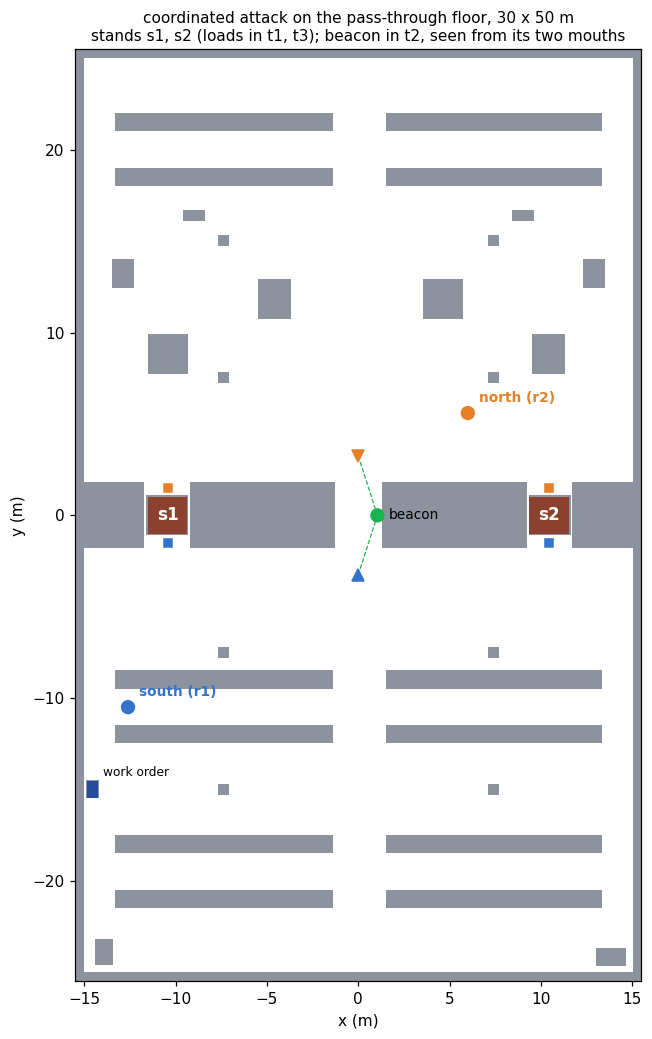
\includegraphics[width=0.52\textwidth]{figures/coordinated_attack_floor.png}
\caption{The floor plan both robots hold. The stands, the beacon and its two
sight lines, the work-order terminal, and where each robot stands under each
load.}
\label{fig:floor}
\end{figure}

The domain makes four claims about the geometry, and the floor generator checks
each on the plan, by casting rays over the occupied cells, before it writes
anything (Table~\ref{tab:geometry}). The third is the one the argument depends
on: two robots under the two ends of one load are three metres apart and cannot
see each other, so meeting at the stand gives no more common knowledge than the
start did.

\begin{table}[H]
\centering\small
\caption{The geometric claims, each checked on the floor plan.}
\label{tab:geometry}
\begin{tabularx}{\textwidth}{@{}X X@{}}
\toprule
claim & what depends on it \\
\midrule
from where they start, neither robot sees the other or the beacon & the radio is the only channel on the radio floor \\
from its viewpoint, each robot sees the beacon & the observability condition of $\mathit{signal}$ \\
under the two ends of one load, the robots do not see each other & meeting at the stand does not replace the beacon \\
every place a robot is sent is reachable over the inflated plan & a correct policy is drivable \\
\bottomrule
\end{tabularx}
\end{table}

Each action is performed by a ROS 2 node, and the model is advanced by the
ePlanSys epistemic state after each one, with Aletheia's own product update.
The executor checks every action's knowledge requirement against the model
before it dispatches the action; for $\mathit{lift}(s_1)$ that requirement is
\code{(C (south north) job\_s1)}.

\begin{table}[H]
\centering\small
\caption{How each action is performed.}
\label{tab:performers}
\begin{tabularx}{\textwidth}{@{}l X@{}}
\toprule
action & performer \\
\midrule
$\mathit{read\text{-}order}$ & south drives to the terminal; the outcome is the work order, given to the node as the warehouse's record \\
messages & the message is put on the receiver's inbox and its arrival awaited, which checks that the designated event is the one that occurred; nothing reports it to the sender \\
$\mathit{go\text{-}view}$ & the robot drives to its mouth of $t_2$, and the beacon is checked to be in line of sight from where it stopped \\
$\mathit{signal}$ & the beacon's tier for the stand is lit, after checking that every robot the model places at a viewpoint has the beacon in line of sight; the node refuses to signal if one does not \\
$\mathit{lift}$ & both robots drive to their mouths of the stand, one start time is fixed for both, each drives in under its end, and the load is raised \\
\bottomrule
\end{tabularx}
\end{table}

%  ======================================================================
\section{Runs}
\label{sec:runs}

Both floors were recorded with the order naming $s_1$, on a $3840 \times 1080$
virtual display with RViz on the left and Gazebo on the right, and composed into
one film whose captions are the lines the runs wrote. The second branch was run
without recording.

\subsection{The radio floor}

\begin{table}[H]
\centering\small
\caption{The radio floor, as the run reported it.}
\label{tab:radio-run}
\begin{tabularx}{\textwidth}{@{}l X r@{}}
\toprule
action & reported & model \\
\midrule
plan & no policy for $\mathit{lifted}$ after 0.2\,s; space exhausted at depth 5 & 2 / 2 \\
$\mathit{read\text{-}order}$ & at the terminal after 12\,s; the order names $s_1$; $e_h$ & 2 / 1, $E^0$ \\
$\mathit{tell}$ & ``$\Kop{south}\job(s_1)$'' delivered & 4 / 1, $E^1$ \\
$\mathit{ack}$ & ``$\Kop{north}\Kop{south}\job(s_1)$'' delivered & 6 / 1, $E^2$ \\
$\mathit{ack2}$ & delivered & 8 / 1, $E^3$ \\
$\mathit{ack3}$ & delivered & 10 / 1, $E^4$ \\
$\mathit{lift}(s_1)$ & knowledge requirement does not hold: \code{(C (south north) job\_s1)} & refused \\
\bottomrule
\end{tabularx}
\end{table}

\noindent
The chains computed from the live model after each message were those of
Table~\ref{tab:ladder}, and the mission confirmed through the epistemic state
that $\Kop{north}\Kop{south}\Kop{north}\Kop{south}\job(s_1)$ held and
$\Cop{G}\job(s_1)$ did not. Neither robot moved toward a stand.

\subsection{The beacon floor}

\begin{table}[H]
\centering\small
\caption{The beacon floor, as the run reported it.}
\label{tab:beacon-run}
\begin{tabularx}{\textwidth}{@{}l X r@{}}
\toprule
action & reported & model \\
\midrule
plan & 8 policy items, 2 leaves, 0.2\,s & 2 / 2 \\
$\mathit{go\text{-}view}(\ag{north})$ & at its viewpoint after 17\,s; beacon in line of sight, 3.5\,m & 2 / 2 \\
$\mathit{read\text{-}order}$ & at the terminal after 12\,s; the order names $s_1$; $e_h$ & 2 / 1, $E^0$ \\
$\mathit{go\text{-}view}(\ag{south})$ & at its viewpoint after 47\,s; beacon in line of sight, 3.5\,m & 2 / 1, $E^0$ \\
$\mathit{signal}(\ag{south}, s_1)$ & in line of sight: south (3.5\,m), north (3.5\,m) & 3 / 1, $C$ \\
$\mathit{lift}(s_1)$ & at the mouths after 22 and 23\,s; joint start; under the load after 13.5 and 13.1\,s: starts 0.00\,s apart, arrivals 0.40\,s apart; load raised 0.12\,m & 1 / 1, $C$ \\
\bottomrule
\end{tabularx}
\end{table}

\noindent
With the order naming $s_2$ the read gave $e_e$, the $s_2$ tier was lit,
$\Cop{G}\job(s_2)$ held, and the load on $s_2$ was raised with arrivals 0.60\,s
apart.

\begin{figure}[H]
\centering
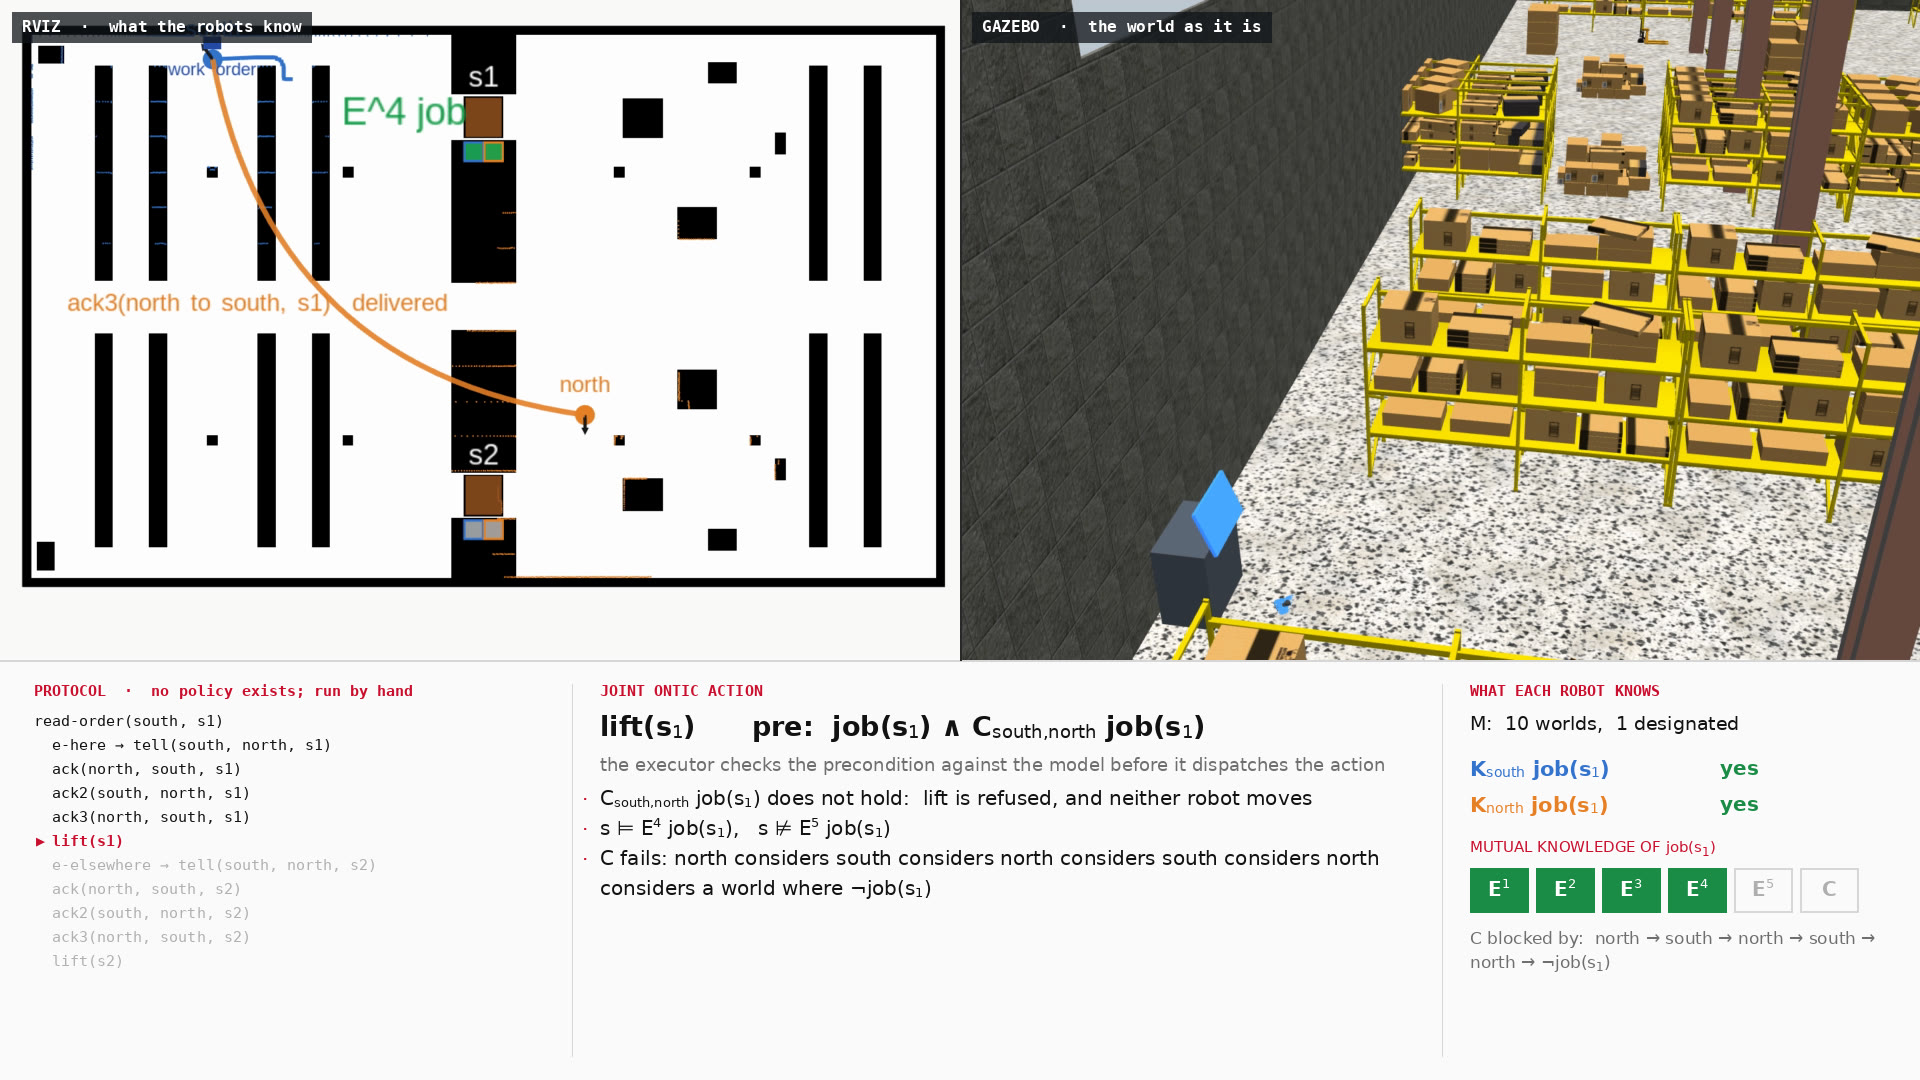
\includegraphics[width=\textwidth]{figures/coordinated_attack_frame_refused.jpg}\\[0.4em]
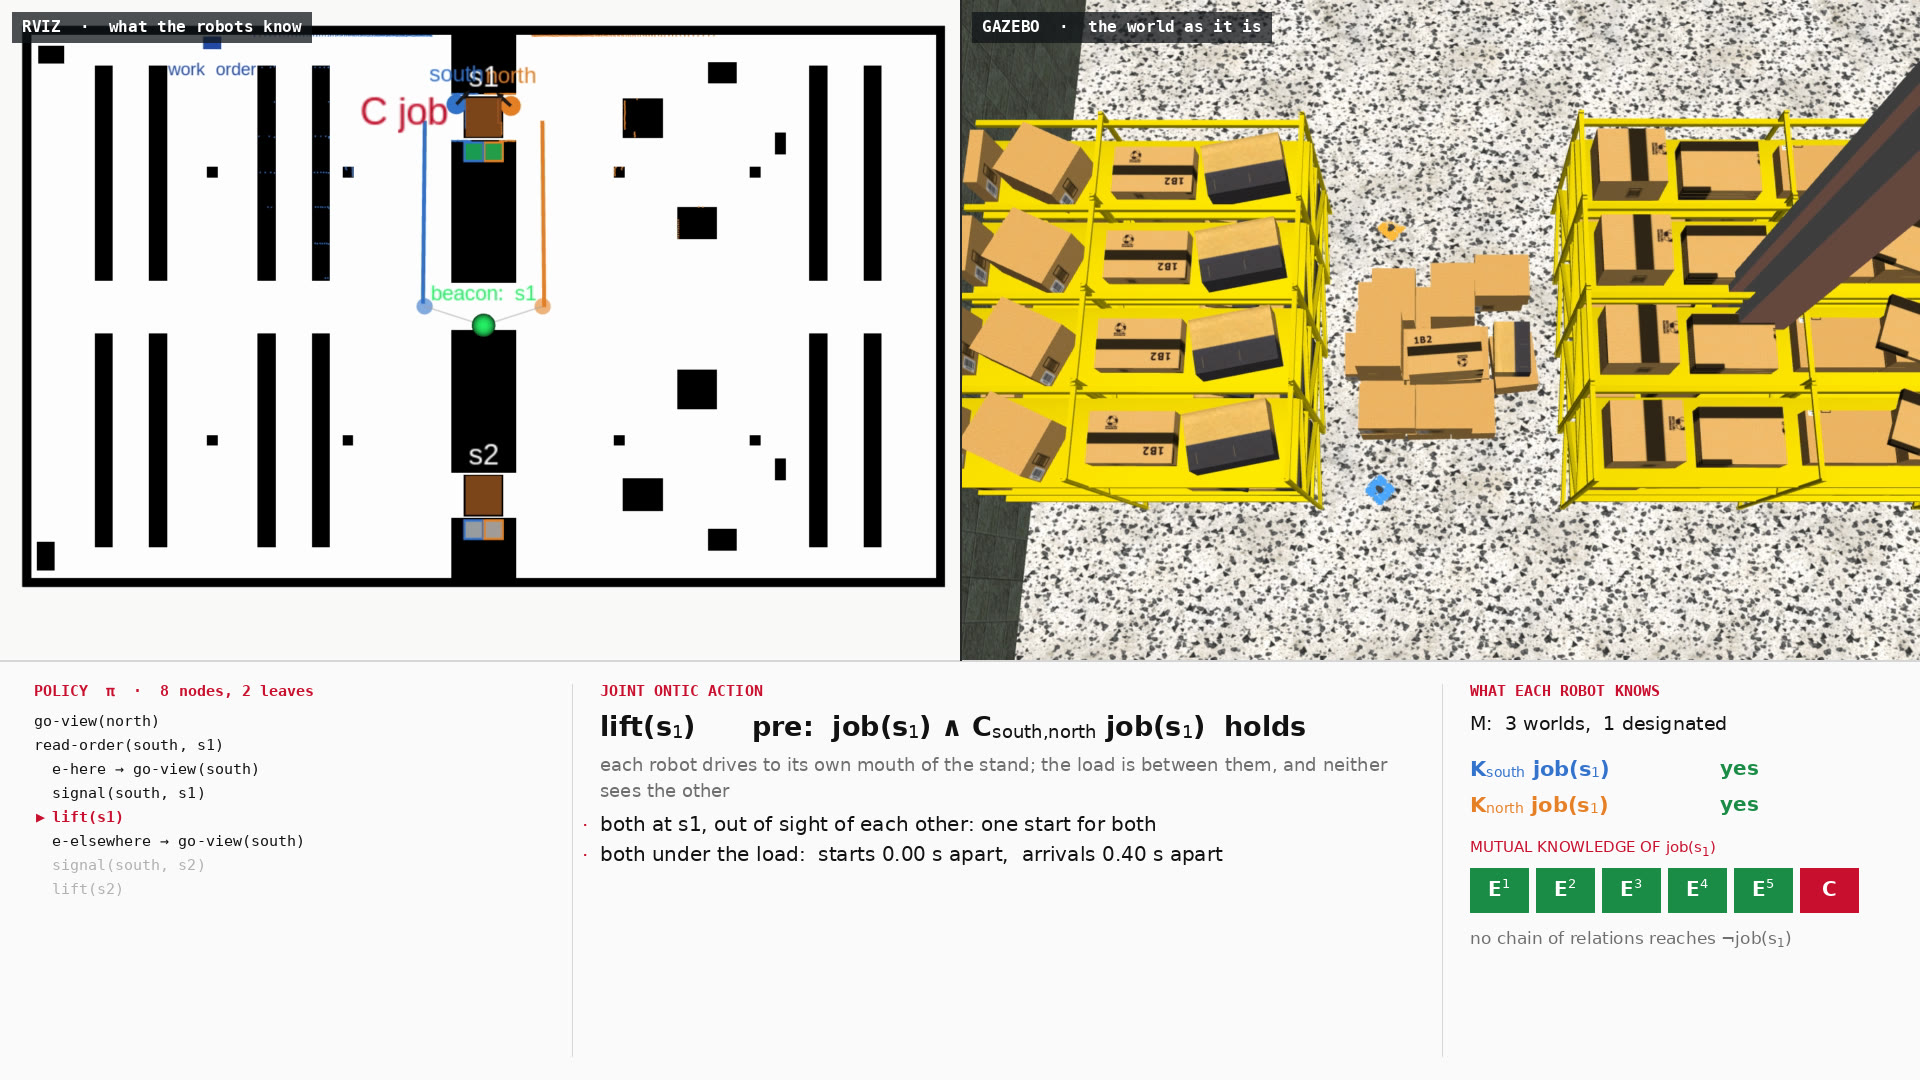
\includegraphics[width=\textwidth]{figures/coordinated_attack_frame_lift.jpg}
\caption{Two frames of the film. Above, the radio floor after the fourth
message: $E^4$, and the lift refused. Below, the beacon floor during the lift,
seen from above the bay: $C$, both robots under the load.}
\label{fig:frames}
\end{figure}

%  ======================================================================
\section{Defects}
\label{sec:defects}

\paragraph{One event named twice is one event} The lost event was first given
by passing the delivered event a second time. plank keys an event model by
event name, so the two became one, the loss disappeared from the model, and the
radio floor was reported unsolvable at depth three for the wrong reason. Each
message now has a lost event of its own.

\paragraph{A signal from the terminal} Before $\mathit{read\text{-}order}$
required $\neg\atview(i)$, the policy sent south to its viewpoint and then to the
terminal, and had it signal from there. The model placed south at its
viewpoint; the line-of-sight check read \code{south no, north yes}. The domain
now orders the two, and the signal node refuses whenever the model and the floor
disagree about who sees the beacon.

\paragraph{A static group modality} A common-knowledge modality over an atom
no action changes requires \code{:static-common-knowledge}, and plank warns
under \code{:common-knowledge}.

\paragraph{Teardown} After the mission reports its result, the action nodes
exit on signal 11 as the launch shuts down. The result is logged first, and the
cause has not been traced.

%  ======================================================================
\section{What the runs establish}
\label{sec:established}

That common knowledge can be stated as the precondition of a joint action and
enforced at execution: the executor evaluated it against the model the
epistemic state maintained, refused the action on the floor where it could not
hold, and dispatched it on the floor where it did.

That the lossy message, as an event model, adds at most one level of mutual
knowledge per message whether or not it is delivered, so that on the radio floor
no policy exists for any number of messages; and that the bound is attained on
the run, four delivered messages yielding $E^4$ and no more.

And that a signal yields common knowledge exactly when each robot's observation
of it is itself common knowledge, which the floor supplies through two
viewpoints and the domain through a public move to them.

%  ======================================================================
\section{Directions for the next iteration}
\label{sec:next}

\paragraph{Positions that must be learned} The domain makes the move to a
viewpoint public. A domain in which robots also learned each other's positions
over the same radio would put the observability condition of the signal itself
out of common knowledge, and Proposition~\ref{prop:public} would no longer
apply.

\paragraph{Probabilistic coordination} Common knowledge is unattainable over a
lossy channel; coordination with a bounded probability of failure is not. A
version in which each robot raises its end after a number of acknowledgements
chosen against a loss rate would trade the precondition for a risk, and would
need the belief layer to state it.

\paragraph{A channel that does fail} The link-outage apparatus gates the topics
a message uses. Composing it with this domain would make delivery an observed
outcome, with both $d$ and $l$ designated and the policy branching on what the
receiver reports.

%  ======================================================================
\begin{thebibliography}{9}
\bibitem{akkoyunlu1975} E.~A. Akkoyunlu, K.~Ekanadham and R.~V. Huber.
  Some constraints and tradeoffs in the design of network communications.
  In \emph{Proceedings of the 5th ACM Symposium on Operating Systems
  Principles}, pages 67--74, 1975.
\bibitem{baltag1998} A.~Baltag, L.~S. Moss and S.~Solecki.
  The logic of public announcements, common knowledge, and private suspicions.
  In \emph{Proceedings of TARK VII}, pages 43--56, 1998.
\bibitem{bolander2011} T.~Bolander and M.~B. Andersen.
  Epistemic planning for single- and multi-agent systems.
  \emph{Journal of Applied Non-Classical Logics}, 21(1):9--34, 2011.
\bibitem{fhmv1995} R.~Fagin, J.~Y. Halpern, Y.~Moses and M.~Y. Vardi.
  \emph{Reasoning About Knowledge}. MIT Press, 1995.
\bibitem{gray1978} J.~Gray.
  Notes on data base operating systems.
  In \emph{Operating Systems: An Advanced Course}, LNCS 60, pages 393--481.
  Springer, 1978.
\bibitem{halpern1990} J.~Y. Halpern and Y.~Moses.
  Knowledge and common knowledge in a distributed environment.
  \emph{Journal of the ACM}, 37(3):549--587, 1990.
\bibitem{vanditmarsch2007} H.~van Ditmarsch, W.~van der Hoek and B.~Kooi.
  \emph{Dynamic Epistemic Logic}. Springer, 2007.
\end{thebibliography}

%  ======================================================================
\section*{Reproduction}

\begin{lstlisting}
ros2 launch coordinated_attack_demo coordinated_attack_launch.py floor:=radio
ros2 launch coordinated_attack_demo coordinated_attack_launch.py floor:=beacon
ros2 launch coordinated_attack_demo coordinated_attack_launch.py order:=s2
bash tools/validate.sh                                   # four checks, no simulator
python3 tools/export_models.py --radio radio.json --beacon beacon.json --out models.json
bash tools/record_demo.sh radio  s1 /tmp/raw_radio.mkv  /tmp/run_radio.log
bash tools/record_demo.sh beacon s1 /tmp/raw_beacon.mkv /tmp/run_beacon.log
python3 tools/make_video.py --radio  /tmp/raw_radio.mkv  /tmp/run_radio.log  /tmp/raw_radio_policy.json \
                            --beacon /tmp/raw_beacon.mkv /tmp/run_beacon.log /tmp/raw_beacon_policy.json \
                            --out /tmp/coordinated_attack.mp4
\end{lstlisting}

\end{document}
